%%%% fs-run-mapreduce Optimistic collision management
\label {fs-collision}

As it was defined previously, only grouping depends on the input order, because it maintains a state. Therefore, we assumed that data items flow through the operations in the right order. However, this restriction is hard to satisfy, because of asynchrony and the possible existence of multiple paths between two nodes.

In order address this issue, we accept the fact that grouping can produce incorrect tuples. However, we guarantee that all correct tuples are eventually produced. The correctness of tuple means that this tuple would be generated if the order assumption was satisfied. 

To eventually produce all correct tuples, we use an approach called {\it replay}. If an item arrives the grouping operation, according to the meta-information order, nothing is replayed and only the most recent window is produced. However, if the item is out of order, it is inserted in the bucket at the correct location, and all tuples, which contain this element, are reproduced. Thereby, replay guarantees that eventually all correct tuples are generated.

The example of replay is shown on the figure~\ref{grouping-replaying-figure}. The colored item is out of order and the window of grouping is 2.

\begin{figure}[htbp]
  \centering
  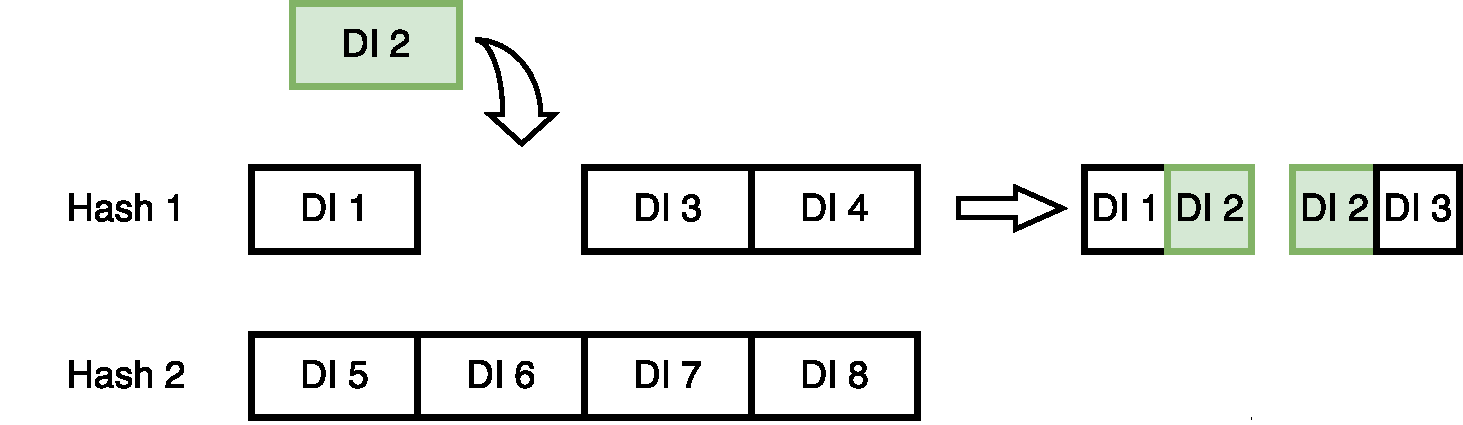
\includegraphics[width=0.48\textwidth]{pics/grouping-replaying}
  \caption{Replay in grouping}
  \label {grouping-replaying-figure}
\end{figure}

In the case of the right order of the input items, there are no redundant items produced. Nevertheless, replay can emit more relevant items, and former ones should not be sent to the outer world.

\subsection{Adaptive microbatching}
In order to filter out invalid elements that are produced on grouping replay, items are collected at barrier before leaving the system.

To differentiate a freshness of items we utilies the structure of meta-information that implements FlameStream ordering model, defined in section~\ref{fs-model}. Then, we introduce an invalidation order on meta that distinguishs correct elements from incorrect ones.

\subsubsection{Meta information}
The meta-information of data item is a pair of a {\it global time} and a {\it trace}.

\[Meta := (GlobalTime, Trace)\]

Global time is assigned to data item once the item enters the system. It is a pair of milliseconds since the epoch start and the identifier of the front. The identifier is used to assign different global times to different items, even in case of wall-clock collisions. 

\[GlobalTime := (FrontTs, FrontId)\]

Global times are compared by front timestamp if they coincide - by front id. It is important to notice, that we are not relying on any clock synchronization between nodes, but we require a strict monotonicity within the single front.

Trace is an array of logical times of operations and the ordinal number of the output within single input which we call {\it child id}. 

\[Trace := [LocalTime]\]

\[LocalTime := (LogicalTime, ChildId)\]

The logical time is a simple item counter within each operation. Therefore, child id is required as map and broadcast can generate multiple items from one. Items with the same child id are called {\it siblings}. When an item leaves an operation, its trace is appended with a new local time. The traces are compared lexicographically.

In spite of the fact that initially there are no items with the same global time, they can be generated by some operations. The trace is used to distinguish two elements with the same global time.

Our concept of meta-information is similar to vector clocks~\cite{fidge1988timestamps, mattern88virtualtime}. However, unlike vector clocks, meta-information provides for the total order of data items due to the global time.

The figure~\ref{logical-graph-ops-figure} shows the topology of each operation and how it affects the trace of local times.

\begin{figure}[htbp]
  \centering
  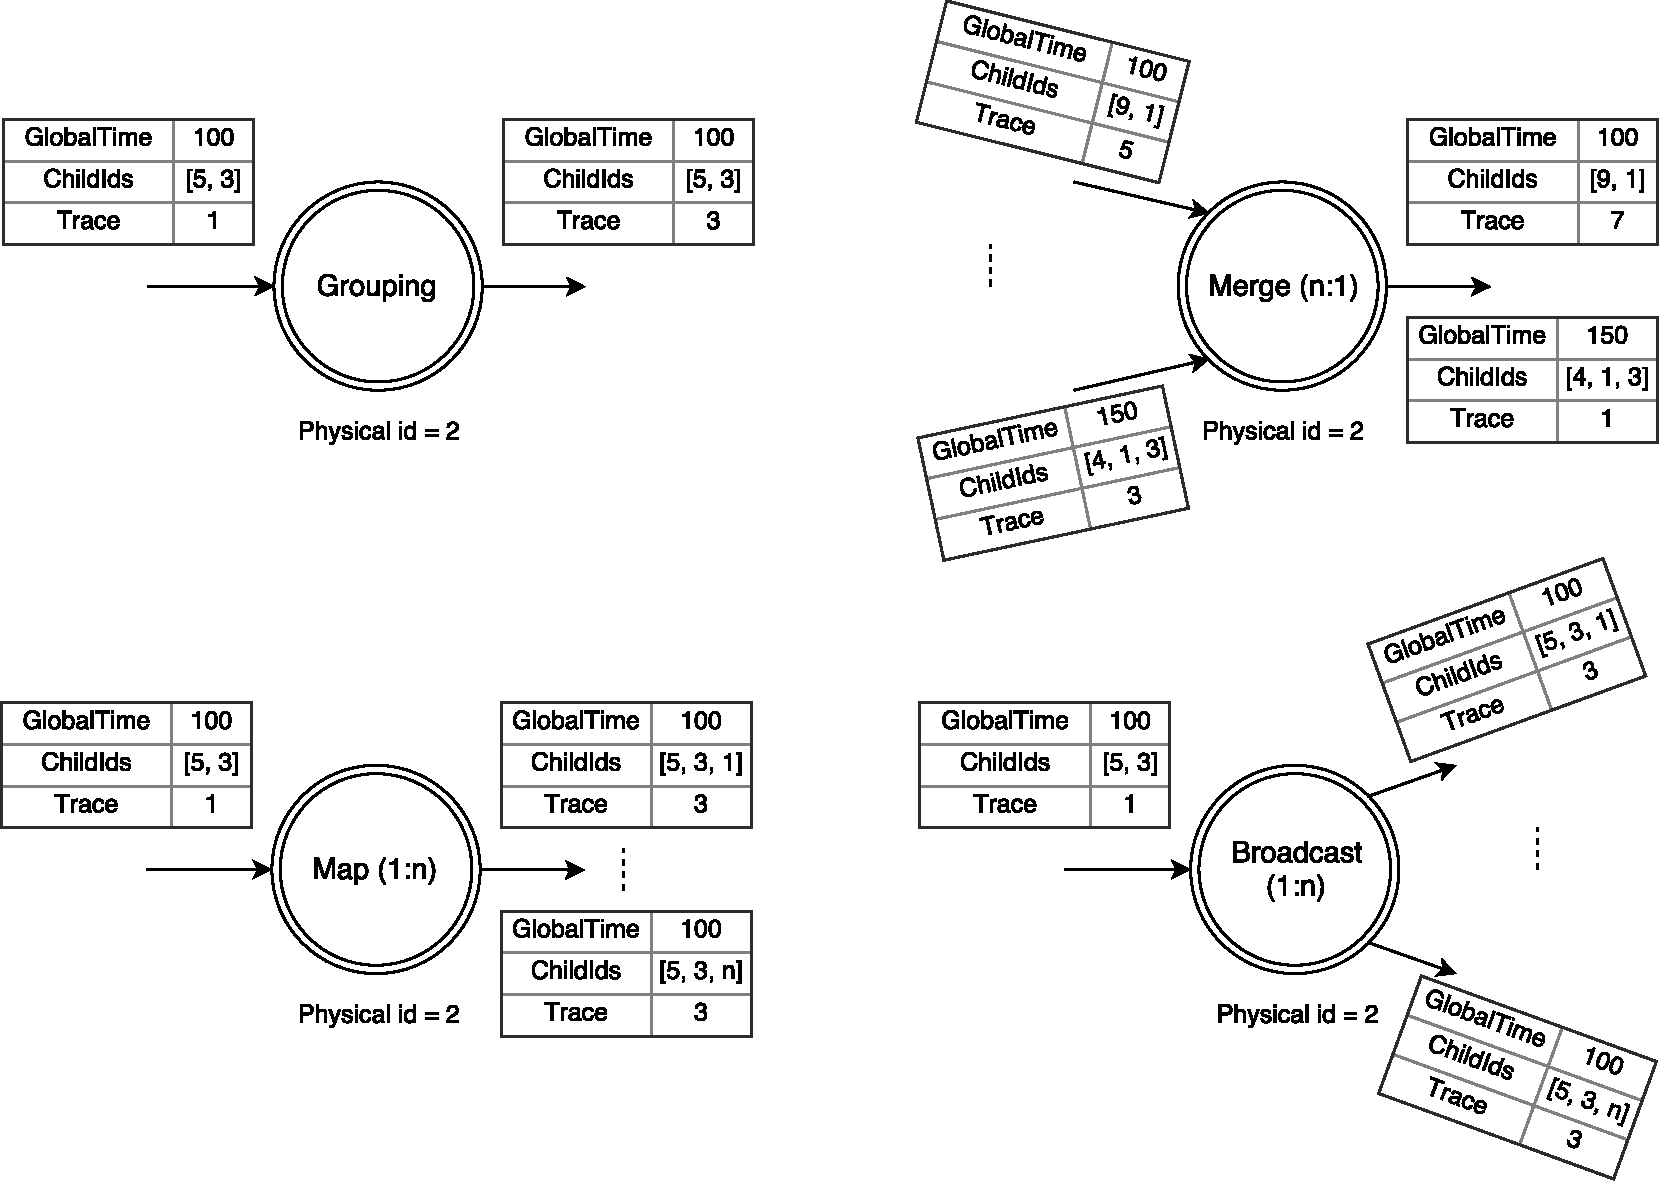
\includegraphics[scale=0.5]{pics/operations}
  \caption{Meta-information handling}
  \label {logical-graph-ops-figure}
\end{figure}

The structure of meta provides for tracking different relations between data items:

\begin{itemize}
  \item{{\it From which elements current one was produced?} From items with common trace prefix.}
  \item{{\it Which element was generated earlier?} One with lower meta.}
\end{itemize}

\subsection{Invalidation mechanism}

Replay in the grouping can generate multiple tuples with the same last item. Only one tuple from such set is correct. To find out which tuples are incorrect we introduce the invalidation rule on data items: if there are several tuples with the same last element, the most recent one is the correct one.

The item {\it A} is said to be invalidated by item {\it B} and {\it B} is called {\it invalidator} of {\it A}, or simply {\it invalidator} iff:

\begin{enumerate}
\item They have the same global time
\item The trace of {\it A} is lexicographically less than the trace of {\it B}
\item The first difference in traces is in logical time
\end{enumerate}

If the first difference is in child id, e.g. they were generated by the broadcast operation, there is no invalidation order between them. Hence, the invalidation order is a partial order. 

Invalidation order is defined not only for the grouping output but for all items. Stateless operations cannot distinguish items thus act on them identically. However, the invalidation order cannot be lost, when an item goes through operations because the trace of local times is append-only.

Barrier maintains a buffer of items. Once a new item arrives, it is inserted into the buffer and items that are invalidated by newcomer are removed. The pseudocode is shown in the alogorithm~\ref{buffer-insert}.

\begin{algorithm}
\caption{Inserting element in buffer}
\label{buffer-insert}
\begin{algorithmic}
  \Function{INSERT}{$a$}
    \ForAll{$item \in buffer$} 
      \If{$item$ is invalidated by $a$} 
        \State \Call{dequeue}{buffer, item}
      \EndIf
    \EndFor
    \State \Call{enqueue}{buffer, a}
  \EndFunction
\end{algorithmic}
\end{algorithm}

There are two complications with invalidation mechanism. The first one, barriers are deployed on multiple workers and are partitioned by the business-logic balancing function. Hence, the item and corresponding invalidator can arrive at distinct barriers. As defined earlier they have the same global time, so the partitioning of barriers by global time solves this problem. The second one, it is unclear when the items should be released from the barrier. The system should ensure that there are no in-flight invalidators. 

The figure~\ref{invalidation-problems-figure} illustrates possible barrier issues. Red items with labels 4 and 7 got out from the system, despite the fact that they should be invalidated by corresponding green items. 

The solution of this problem is described in the next subsection. 

\begin{figure}[htbp]
  \centering
  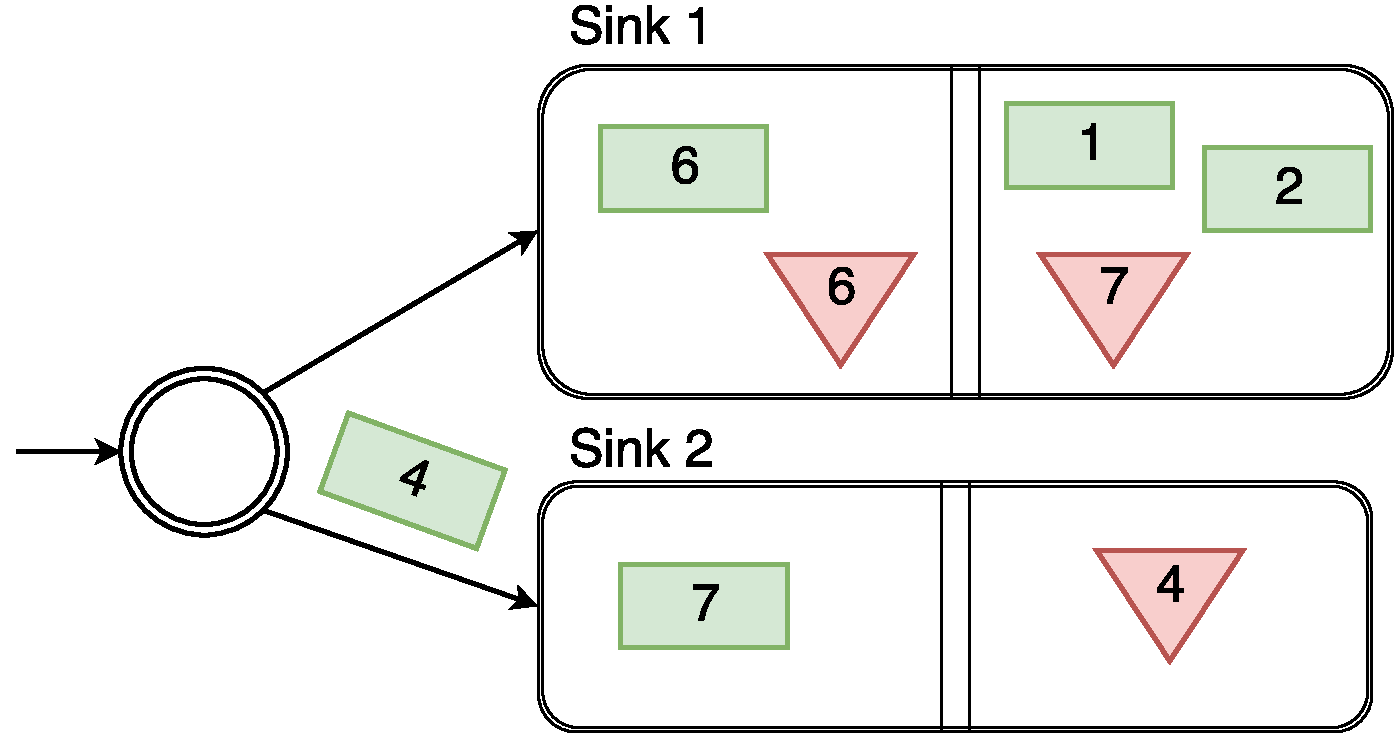
\includegraphics[width=0.48\textwidth]{pics/invalidation_problems}
  \caption{Possible barrier issues}
  \label {invalidation-problems-figure}
\end{figure}

\subsection{Minimal time within stream}

To release the item from the barrier we need to ensure that there are no in-flight invalidators. 

\newtheorem{minimal-time-claim}{Lemma}

\begin{minimal-time-claim}
  If data item {\it D} has global time {\it GT} greater than the global time of the in-flight elements, then all items that could invalidate {\it D} had already arrived at the barrier.
\end{minimal-time-claim}

\begin{proof}
  Let {\it E} is in-flight element that invalidates {\it D}. According to the definition of invalidation order, {\it E} and {\it D} have the same global time {\it GT}, but the different trace. We assumed that there are no in-flight element with the global time equal to {\it GT}. Contradiction.

  This implies that if the stream does not contain items with the global time less than or equal to {\it GT}, then all items which invalidate {\it D} had already arrived at the barrier. 
\end{proof}

Therefore, to output an item from the barrier, we should ensure that there are no items in the stream with global time less than or equal to the global time of this item.

To track the global time of in-flight items we adopt an idea of {\it acker task} borrowed from Apache Storm~\cite{apache:storm}. Acker tracks data items using a checksum hash. When the item is sent or received by an operation, its global time and checksum are sent to the acker. This message is called {\it ack}. Acker groups acks by a global time into the structure called {\it ack table}. Once acker receives an ack message with global time {\it GT} and {\it XOR} it updates {\it GT} entry in the table by xoring {\it XOR} with the current value. When an item is sent and later received by the next operation, xoring corresponding {\it XOR}s would yield zero.

Acks are overlapped to nullify table's entry only when an item arrives at the barrier. That is, ack for receive is sent only after both processing and the ack sending for the transformed item, as illustrated in the figure~\ref{acker}. Different colors of items mean different payloads. The ack for the sending of the blue element is sent before the green one. We expect the channel between the acker and each operation to be FIFO, so ack for the blue item would be xored before the green. So the two equal values are separated by distinct one. 

This technique guarantees that the {\it XOR} for some global time is equal to zero only if there are no in-flight elements with such global time.

\begin{figure}[htbp]
  \centering
  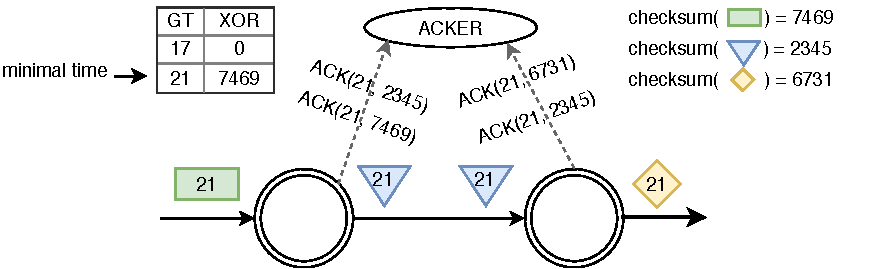
\includegraphics[scale=0.5]{pics/acker}
  \caption{Acker}
  \label {acker}
\end{figure}

The minimal time within a stream is the minimal global time with non-zero {\it XOR}. On minimal time changes, acker broadcasts new minimal time to the barrier and operations. Therefore, the barrier can release elements with global time {\it GT} once it received notification from acker that the minimal time within the stream is greater than {\it GT}.

To ensure that no fronts are able to generate item with the certain timestamp, each front periodically sends to acker special message called {\it report}, which promise to generate items with the greater timestamp. The value in the ack table can become a zero only after the corresponding report arrives.

The proposed mechanism could be isolated by hash range. This change allows us making invalidation and releasing from barrier independent also known as key readiness.
